\section{Retention quality and design sensitivity}
\label{sec:supp_quality}
We examine how pruning layer, retention budget, and scoring rule affect quality on the inspected ScanQA split. Replay and sensitivity analyses assess these choices within the development setting. Selection stability and local multiplicity corrections neither provide independent confirmation nor account for the complete historical search.


\subsection{Schedule controls}
The schedule grid includes FastV-style L2/R10, PyramidDrop-style drops at L8/16/24 with cumulative ratios 0.50/0.25/0.125, and an AdaToken-inspired exponential-decay approximation. EM values are 23.04, 27.25, and 26.95, respectively, versus 27.79 for GeoGate.

The main-text FastV-style comparison instead uses L2/R50. Its GeoGate-minus-control scene intervals are $[0.55,2.02]$ EM and $[2.06,5.87]$ CIDEr. For PyramidDrop, the corresponding intervals are $[0.00,1.12]$ and $[-1.29,2.31]$; for AdaToken, they are $[0.29,1.41]$ and $[-0.01,2.98]$. These are implemented schedule controls rather than official reproductions. Relative to native, the headline R10 question-level EM interval is $[-0.02,0.92]$, with 77 wins, 4542 ties, and 56 losses.

\Cref{sec:supp_baseline_availability} documents related implementation availability.

\subsection{Shared-input layer replay}
\label{sec:supp_layer_replay}

Shared-input replay tests whether the original layer ordering persists when every condition shares the same prepared inputs. The original 11-layer curve (\cref{fig:supp_original_layer_curve}) contains frozen aggregate values without per-question artifacts. We repeat the sweep on the same inspected 4,675-question, 71-scene ScanQA validation split, sharing each question's video tensor and expanded embedding across conditions. All pruning arms use $R=0.10$, head-averaged last-prompt attention, greedy decoding, and the frozen per-question seed. The main-text paired replay reports this runner's means and simultaneous contrast intervals. \Cref{tab:supp_layer_replay} preserves both runners' values. Neither evaluation is an independent holdout.

\begin{table}[t]
\centering
\caption{Original aggregate curve (\cref{fig:supp_original_layer_curve}) versus the shared-input replay shown in the main text. Both columns are ScanQA EM on the inspected split.}
\label{tab:supp_layer_replay}
\resizebox{\columnwidth}{!}{%
\begin{tabular}{rrrr}
\toprule
Layer & Original EM & Replay EM & Difference \\
\midrule
L2 & 23.0400 & 22.8021 & $-0.2379$ \\
L4 & 22.4800 & 22.5241 & $+0.0441$ \\
L6 & 23.3600 & 23.2513 & $-0.1087$ \\
L8 & 25.0100 & 24.8984 & $-0.1116$ \\
L10 & 26.4400 & 26.3529 & $-0.0871$ \\
L12 & 27.1700 & 26.9947 & $-0.1753$ \\
L13 & 26.9700 & 26.9091 & $-0.0609$ \\
L14 & 27.7900 & 27.7219 & $-0.0681$ \\
L15 & 27.5900 & 27.5936 & $+0.0036$ \\
L16 & 27.3800 & 27.4652 & $+0.0852$ \\
L18 & 27.5300 & 27.5294 & $-0.0006$ \\
\bottomrule
\end{tabular}}
\end{table}

Replay preserves the low-attention interval's trough, the rise through L8--L12, and the late plateau; the largest absolute difference is 0.2379 EM points. L14 is the highest measured point in both versions. Scene-clustered studentized max-$t$ intervals compare L14 against the other 11 measured conditions and support L14 advantages within this family. The analysis uses 10,000 draws and seed 20260920, with simultaneous critical value 2.7202 and familywise $p=0.0001$. L14 exceeds L2/L4/L6/L8/L10/L12/L13 with simultaneous intervals wholly above zero. The remaining contrasts are unresolved: L14 minus native is $+0.2995$ $[-0.4100,+1.0089]$, L14 minus L15 is $+0.1283$ $[-0.3499,+0.6066]$, L14 minus L16 is $+0.2567$ $[-0.3508,+0.8642]$, and L14 minus L18 is $+0.1925$ $[-0.4517,+0.8367]$.

These results support L14 as a representative point on a late quality plateau. They do not establish superiority over the unpruned model or neighboring L15/L16/L18 conditions.

\begin{figure}[t]
\centering
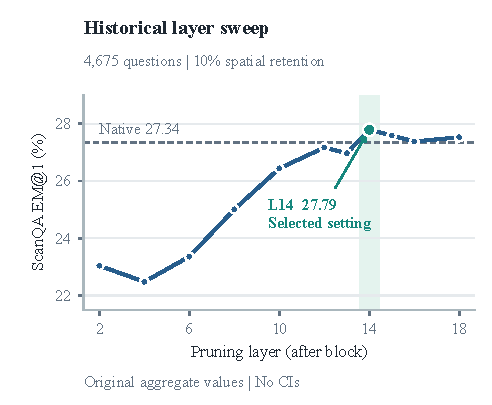
\includegraphics[width=\columnwidth]{fig_layer_curve.pdf}
\caption{Original aggregate ScanQA layer values. The native baseline is 27.34 and L14 is 27.79, without per-question intervals. The main-text paired-replay figure uses its own native 27.4225/L14 27.7219 values and frozen simultaneous contrast intervals. Intervals remain specific to their runner.}
\label{fig:supp_original_layer_curve}
\end{figure}

\subsection{Retention budget}
\label{sec:supp_keep_ratio}

The tested retention ratios yield similar point estimates in the complete 4,675-question sweep at L14 (\Cref{tab:supp_ratio}). Every paired scene-level EM interval relative to the runner-matched baseline includes zero. The default 10\% ratio was chosen from joint validation-set point estimates and is not statistically superior to 5\% or 20\%.

We assess selection stability using a scene-level leave-one-out rule on the same frozen predictions. Each fold selects the budget using the other 70 scenes and evaluates it on the held-out scene. The rule selects 10\% in 68/71 folds. Held-out-selected EM is 27.57, versus 27.79 for fixed 10\%, with a scene-bootstrap difference of $-0.21$ $[-0.50,0.00]$.

\begin{table}[t]
\centering
\caption{Keep-ratio sensitivity on LLaVA-3D ScanQA validation.}
\label{tab:supp_ratio}
\begin{tabular}{lccc}
\toprule
Kept & EM@1 & CIDEr & EM delta 95\% CI \\
\midrule
5\% & 27.72 & 93.12 & [-0.22, 1.01] \\
10\% & 27.79 & 94.33 & [-0.07, 0.99] \\
20\% & 27.68 & 94.32 & [-0.04, 0.73] \\
\bottomrule
\end{tabular}
\end{table}

\subsection{Token-scoring rules}
\label{sec:supp_scorers}

At L14, last-prompt and prompt-mean attention yield higher EM point estimates than the tested random, norm, CLS-attention, and entropy alternatives (\Cref{tab:supp_scorer}). Each scorer is compared at the stated pruning depth. The grid is incomplete, and missing entries are not imputed. A fixed scoring formula can select different token identities across layers, so this comparison does not isolate a depth-only effect.

\begin{table}[t]
\centering
\caption{Scoring-rule comparison at 10\% retention.}
\label{tab:supp_scorer}
\begin{tabular}{lcc}
\toprule
Scorer & L2 EM@1 & L14 EM@1 \\
\midrule
Last-prompt attention & 23.04 & 27.79 \\
Prompt-mean attention & --- & 27.66 \\
Random & 24.77 & 25.67 \\
Token L2 norm & 19.34 & 25.22 \\
CLS attention & 21.22 & 23.23 \\
Attention entropy & --- & 23.23 \\
\bottomrule
\end{tabular}
\end{table}

\subsection{Analytical-cost-matched layer controls}
\paragraph{Selection stability.} Layer selection is stable within the frozen cost-matched runner. Each fold chooses among L2-matched, L8-matched, and L14/128 conditions using the other 70 scenes, then evaluates the selected condition on the held-out scene. L14/128 is selected in 71/71 folds, with a scene-bootstrap selection probability of 0.9984. Nested-selected and fixed-L14/128 EM are both 27.8930, with a difference of 0.0000 $[0.0000,0.0000]$. Unadjusted held-out scene counts are 38/17/16 better/equal/worse for L14 against L2 and 33/17/21 against L8. The scene counts are exploratory.

\paragraph{Scene robustness.} Both prespecified cost-matched contrasts retain positive effects when any complete scene is removed. Using frozen per-question exact-match outcomes, the L14/128 leave-one-scene-out range is $1.0206$--$1.3069$ EM points against L2 and $0.8903$--$1.1206$ against L8. Unadjusted discordant-question counts are 140/83 better/worse against L2 and 144/96 against L8. Their exact two-sided sign-test values are $1.64\times10^{-4}$ and $2.35\times10^{-3}$; Holm correction over the two contrasts gives $3.28\times10^{-4}$ and $2.35\times10^{-3}$. Corresponding scene-mean directions are 38/17/16 and 33/17/21 better/tie/worse.

The sign tests are post-hoc diagnostics and do not replace the prespecified scene-bootstrap intervals for L14/128.

\subsection{Multiplicity within restricted candidate families}
\Cref{tab:supp_max_t} examines selection sensitivity within two frozen three-candidate families. A scene-clustered studentized max-$t$ correction covers all three pairwise contrasts within each family, without reconstructing the complete historical search.

\begin{table*}[t]
\centering
\small
\caption{Limited max-$t$ correction for the frozen layer and budget families. Intervals are 95\% simultaneous intervals over all pairwise contrasts within each stated three-candidate family.}
\label{tab:supp_max_t}
\begin{tabular}{lccc}
\toprule
Family & Contrast & EM points & Max-$t$ 95\% CI \\
\midrule
Layer & L14/128 $-$ L2 cost-matched & $+1.2193$ & $[0.3242,2.1143]$ \\
Layer & L14/128 $-$ L8 cost-matched & $+1.0267$ & $[0.1707,1.8828]$ \\
Layer & L8 cost-matched $-$ L2 cost-matched & $+0.1925$ & $[-0.6284,1.0134]$ \\
Budget & R=0.10 $-$ R=0.05 & $+0.0642$ & $[-0.4565,0.5849]$ \\
Budget & R=0.10 $-$ R=0.20 & $+0.1070$ & $[-0.3317,0.5456]$ \\
Budget & R=0.20 $-$ R=0.05 & $-0.0428$ & $[-0.6353,0.5498]$ \\
\bottomrule
\end{tabular}
\end{table*}

The layer family retains positive intervals after correction, with familywise max-$t$ $p=0.0062$ and critical value 2.3275. The L8-minus-L2 control remains unresolved. All three budget contrasts remain unresolved, with $p=0.8458$ and critical value 2.3286. The two cost-matched L14/128 advantages therefore survive this limited three-candidate correction. R=0.10 remains representative of a quality plateau rather than a unique optimum.

The correction covers only the six listed contrasts, excluding other layers, scorers, budgets, prompts, and thresholds inspected during development. It does not estimate performance under the full historical search.

\subsection{Bootstrap-seed sensitivity}
All six primary paired endpoints retain positive intervals across the tested bootstrap seeds (\Cref{tab:supp_primary_seed}). These endpoints comprise two cost-matched EM contrasts, two first-token log-probability contrasts, and two complete-answer EM contrasts. Each uses the original scene-cluster bootstrap seed and four deterministic offsets, with 10,000 resamples per seed. All six endpoints retain a positive 97.5\% interval under all five seeds, with unchanged point estimates.

\begin{table*}[t]
\centering
\small
\caption{Bootstrap-seed sensitivity for the six primary paired endpoints. The interval range is the union of the five 97.5\% intervals.}
\label{tab:supp_primary_seed}
\begin{tabular}{lccc}
\toprule
Endpoint & Point estimate & Interval range & Stable \\
\midrule
Cost-matched L14$-$L2 EM & 1.2193 & [0.3882, 2.1432] & 5/5 \\
Cost-matched L14$-$L8 EM & 1.0267 & [0.2168, 1.8734] & 5/5 \\
First-token L14$-$L8 & 0.2513 & [0.2108, 0.2965] & 5/5 \\
First-token L14$-$L20 & 0.2159 & [0.1779, 0.2573] & 5/5 \\
Complete-answer L14$-$L8 EM & 3.2014 & [1.7435, 4.7267] & 5/5 \\
Complete-answer L14$-$L20 EM & 2.9733 & [1.8217, 4.2263] & 5/5 \\
\bottomrule
\end{tabular}
\end{table*}

The prespecified seed remains the primary analysis; these post-hoc reruns assess Monte Carlo sensitivity only.

\subsection{Cross-layer scoring and adaptive onset}
Cross-layer score aggregation provides no resolved benefit at the selected L14 configuration. On LLaVA-3D, stable attention obtains 27.55 EM and 93.82 CIDEr, changing EM by $-0.24$ with scene-level 95\% CI $[-0.57,0.10]$. On 3D-LLaVA, windows 2, 3, and 5 likewise have point estimates below single-layer scoring, with intervals containing zero (\Cref{tab:supp_stable}). These comparisons establish neither an improvement nor the absence of an effect.

\begin{table}[t]
\centering
\caption{Stable-attention scoring on 3D-LLaVA ScanQA, L14, 10/100 tokens.}
\label{tab:supp_stable}
\resizebox{\columnwidth}{!}{%
\begin{tabular}{lccc}
\toprule
Scorer & EM@1 & CIDEr & EM delta scene 95\% CI \\
\midrule
Single-layer & 27.83 & 90.42 & --- \\
Window 2 & 27.57 & 89.80 & [-0.64, 0.13] \\
Window 3 & 27.70 & 89.95 & [-0.49, 0.22] \\
Window 5 & 27.66 & 89.80 & [-0.60, 0.26] \\
\bottomrule
\end{tabular}}
\end{table}

Adaptive onset changes pruning depth, but neither variant establishes quality preservation (\Cref{tab:supp_adaptive}). Resetting detector state for each sample produces non-degenerate layer distributions for both variants. The default detector triggers later than fixed L14 on average. The shared detector triggers earlier but has not passed a prespecified non-inferiority test. Historical latency values were collected in separate sessions and are excluded from comparative timing claims.

\begin{table}[t]
\centering
\caption{Corrected adaptive-onset evaluation on LLaVA-3D ScanQA.}
\label{tab:supp_adaptive}
\resizebox{\columnwidth}{!}{%
\begin{tabular}{lcccc}
\toprule
Schedule & Mean layer & Median & EM@1 & CIDEr \\
\midrule
Fixed L14 & 14.00 & 14 & 27.79 & 94.33 \\
Adaptive default & 16.71 & 18 & 27.61 & 94.09 \\
Adaptive shared & 12.75 & 12 & 27.47 & 93.22 \\
\bottomrule
\end{tabular}}
\end{table}

\subsection{Exploratory geometry and coverage}
Both coverage-aware variants score below the attention reference, but their prompt mismatch prevents attributing this difference to the selector (\Cref{tab:supp_coverage}). The selector preserves the highest-attention token, then greedily balances attention against minimum distance to the selected set using OST superpoint centroids. Unit tests verify coordinate alignment, uniqueness, budget clamping, and top-$K$ fallback for invalid coordinates.

Both full-set variants use the original unsuffixed ScanQA prompt. The attention reference uses ``Answer the question simply.'' on the same 4,675 questions. This prompt mismatch prevents interpreting the score differences as paired selector effects. Neither variant is used in GeoGate. The pilot evaluates this greedy selector in the tested 3D-LLaVA runner; it does not reproduce CoVeR's coordinate-covering selector for multi-view 2D VLMs. Its results do not establish that coverage-based selection is generally ineffective.

\begin{table}[t]
\centering
\caption{Unmatched-prompt coverage pilot on 3D-LLaVA ScanQA.}
\label{tab:supp_coverage}
\resizebox{\columnwidth}{!}{%
\begin{tabular}{lccc}
\toprule
Selector & EM@1 & CIDEr & Pairing \\
\midrule
Attention top-$K$ reference & 27.83 & 90.42 & suffixed prompt \\
Stable + coverage, 0.25 & 25.50 & 82.00 & unsuffixed prompt \\
Attention + coverage, 0.10 & 25.48 & 82.45 & unsuffixed prompt \\
\bottomrule
\end{tabular}}
\end{table}

Additional 500-question pilots do not support adopting geometry diffusion or coarsening. Neighbor diffusion overlaps the attention-only pilot range. Mean-pooling discarded tokens into 16 or 64 contiguous or voxel-aware groups yields no point-estimate improvement over deletion and has higher recorded latency. These bounded diagnostics support neither full-set conclusions nor a general absence of benefit.
